\section{Introduction}
%
Every industrial and enterprise sector in our society is either
actively using Large Language Models (LLMs) or eager to adopt
them~\cite{intro_1, intro_2}.
%
LLM's widespread success can be attributed to the effectiveness of
their core algorithmic component,
\emph{transformers}~\cite{vaswani2023attention}.
%

%
While transformers offer remarkably versatile capabilities and continue to
dominate LLMs, their enormous resource demands are a significant
concern for LLM providers.
%
Transformer-based LLMs scale quadratically in compute and linearly in
memory footprint with sequence length, while emerging
applications--such as test time scaling~\cite{deepseekr1, googletts,
o1, s1}, retrieval-augmented generation~\cite{rag, pmlrrag, copy,
toolformer}, and multimodal input fusion~\cite{gpt4o, llama4}--are
driving demand for longer sequence lengths, recently reaching up to 2
billion tokens in industry-leading models~\cite{longrope}.
%
Moreover, batched inferencing exacerbates these resource demands,
forcing hyperscalers to invest billions of dollars in equipping their
data centers with hundreds of thousands of costly GPUs, each priced
at \$30,000 or more~\cite{meta-h100-purchase}.

\begin{figure}[t]
  \centering
  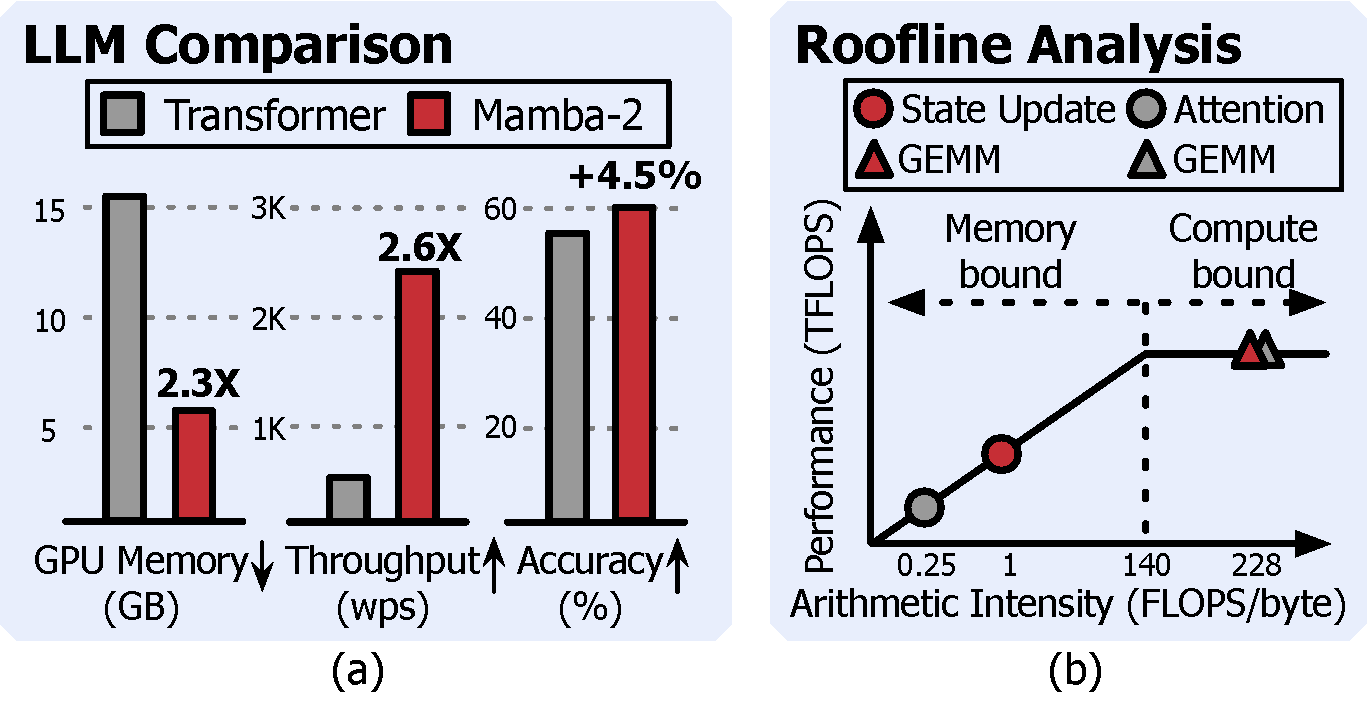
\includegraphics[width=0.95\linewidth]{fig/mamba_vs_transformer.pdf}
  \caption{Comparison between 2.7B parameter transformer and Mamba-2.
  Accuracy results are referenced from~\cite{mamba2}.}
  \label{fig:mamba_vs_transformer}
\end{figure}

%
Recently, the algorithm community has actively explored alternative
approaches, including state space models (SSMs), linear attention
mechanisms, and recurrent neural networks (RNNs).
%
In this paper, we henceforth refer to LLMs employing these
alternative algorithmic techniques as ``post-transformer'' LLMs.
%
We argue that post-transformer LLMs have the potential to serve as a
promising complement to transformer-based LLMs, providing comparable
algorithmic capabilities with significantly lower and constant
resource demands~\cite{mamba, mamba2, s4, h3, hyena, s4d, hippo,
  lssl, linear_attention, gated_linear_attention, gsa, retnet, rwkv,
rwkv6, xlstm, hgrn2}.
%
Figure~\ref{fig:mamba_vs_transformer}(a) presents an empirical
evidence that supports our argument.
%
The figure compares the memory usage, throughput, and accuracy of a
transformer-based LLM with a post-transformer LLM, Mamba-2, both
having a model size of 2.7 billion parameters\footnote{Detailed
experimental methodology is presented in Section~\ref{sec:method}}.
%
The results show that Mamba-2 requires 2.3$\times$ less memory
capacity, delivering 2.6$\times$ higher throughput than the
transformer counterpart, while achieving 4.5\% higher accuracy.
%
Despite this considerable potential, the architecture and system
community have a limited understanding of the implications of these
algorithms, causing LLM providers to hesitate in adopting
them for their serving systems.
%

%
To this end, this paper sets out to bridge this gap through a
comprehensive workload analysis and performance characterization, and
to devise a solution that leverages the resulting insights.
%
The first of these insights is that many post-transformer LLMs share a
common algorithmic operation, \emph{state update}, which propagates
and evolves contextual information across tokens.
%
This commonality offers a promising opportunity for architectural
generalization and acceleration.
%
We also discovered that similar to the attention operation in
transformer-based LLMs, this state update operation becomes the
performance bottleneck due to its low arithmetic intensity.
%
Figure~\ref{fig:mamba_vs_transformer}(b) reports the roofline
analysis results that the arithmetic intensity of state update
operation is 4$\times$ larger than that of attention, while it is
still significantly bandwidth-bound.
%

%
Inspired by these insights, we propose \sysname{}, an acceleration
solution that addresses the memory bandwidth bottleneck by jointly
exploiting (1) Processing-in-Memory (PIM) paradigm, and (2) LLM quantization.
%
While prior works have extensively investigated these techniques for
transformer-based LLM serving~\cite{xiao2023smoothquant,
  hooper2024kvquant, monkey, atom, heo2024neupims,
park2024attacc,ianus}, we observe that post-transformer LLMs
demonstrate significantly different behaviors, requiring distinct
design choices to enable a unified serving system that accommodates
the two classes of LLM architectures.
%
Below, we share the empirical insights and their corresponding
principles that govern our accelerator design:
%
\begin{itemize}[labelindent=0.5em,nolistsep,leftmargin=1.0em]
    %
  \item \textbf{(Principle 1): Maximizing hardware resource sharing
    for area efficiency:}
    %
    Existing LLM-targeted PIM acceleration methods~\cite{hbm_pim,
    newton, heo2024neupims, park2024attacc, ianus} focus on
    supporting matrix-vector multiplication (i.e., GEMV) since
    attention operation consists of a full of GEMVs.
    %
    However, this approach is unsuitable for post-transformer
    algorithms since implementing the state update operation in
    hardware incurs significantly larger area costs due to the
    variety of primitives in state update operation, such as
    element-wise multiplication, element-wise addition, and vector dot products.
    %
    Thus, in designing \sysname{}, we aim to exploit the hardware
    resource sharing for maximizing area efficiency.
    %
  \item \textbf{(Principle 2): Achieving both accuracy and
    area-efficiency from low-precision arithmetic:}
    %
    While quantizing the \emph{state} in post-transformers can reduce
    computation cost and memory footprint, it also affects area efficiency.
    %
    We also discover that, due to the state ``update’’ mechanism,
    conventional numerical formats cause severe accuracy degradation,
    rendering them impractical for post-transformers.
    %
    We carefully explore the accuracy-area tradeoffs and observe that
    different low-precision arithmetic approaches exhibit different
    characteristics.
    %
    We thoroughly perform an empirical study to understand the
    differences and aim to employ a Pareto-optimal quantization
    technique for our solution.
    %
\end{itemize}
%

%
\noindent Building upon these two principles, we design the \sysname{}
accelerator architecture, which incorporates the following key elements:
%

%
\niparagraph{State-update Processing Unit (SPU).}
%
At the core of \sysname{} is the State-update Processing Unit (SPU),
which includes a State-update Processing Element (SPE).
%
Deploying an SPE for each bank would incur excessive area costs and
reduce memory capacity, rendering this approach impractical under the
stringent area constraints of PIM compute units.
%
To address this, \sysname{} assigns one SPU to every two banks.
%
The SPU alternates between reading from and writing to the row
buffers of different banks, performing computations in an interleaved manner.
%
This design sustains throughput while optimizing area efficiency.
%

%
\niparagraph{SPE with MX-based quantized arithmetic.}
%
Empirical analysis suggests that among various quantization formats,
MX8~\cite{rouhani2023shared} (requiring an average of 8 bits per
value) emerges as a Pareto-optimal choice in the accuracy-efficiency
tradeoff, while aligning seamlessly with memory address alignment requirements.
%
This enables area- and power-efficient implementation of SPEs within
the constraints of PIM.
%
Consequently, we design custom MX8 vector multipliers and adders,
significantly improving resource efficiency.
%

%
\niparagraph{End-to-end \sysname{} system design.}
%
We construct the \sysname{} system by jointly leveraging \sysname{}
accelerators with GPUs, offloading state update and attention
operations to PIM, while delegating other tasks to GPUs.
%
\sysname{} includes custom DRAM commands and command scheduling
techniques to manage state pre-charging and subsequent generative computations.
%
Our PIM accelerator and its interface use a system architecture
similar to the existing PIM-based LLM serving
systems~\cite{heo2024neupims, park2024attacc, ianus, cxl-pnm},
allowing \sysname{} to serve as a ``drop-in replacement'' in
transformer-serving systems adapted to support post-transformer LLMs as well.
%

%
To evaluate \sysname{}'s effectiveness, we use four post-transformer
LLM models--Mamba-2, GLA, RetNet, and HGRN2~\cite{mamba2,
gated_linear_attention, retnet, hgrn2}-- along with Zamba2, a hybrid
transformer-Mamba-2 model~\cite{zamba2}, and OPT~\cite{zhang2022opt},
a traditional attention-based model.
%
Our experimental results show that compared to LLM-optimized GPU and
GPU+PIM systems, \sysname{} achieves 14.6$\times$ and 6.9$\times$
lower latency in state update operations, resulting in up to
4.1$\times$ and 2.1$\times$ higher throughput, respectively, with
minimal area overhead on the memory device.
%
These advantages in both performance and area-efficiency demonstrate
that \sysname{} is an effective PIM-based solution for LLM serving,
capable of supporting both transformer and post-transformer models,
paving the way toward scalable and cost-efficient deployment of
emerging LLM architectures.
%
A full-system simulator for \sysname{} and the accuracy evaluation code
are open-sourced at \bluetext{\url{https://github.com/casys-kaist/pimba}}.
%
